%%%%%%%%%%%%%%%%%%%%%%%%%%%%%%%%%%%%%%%%%%%%%%%%%%%%%%%%%%%%%%%%%%%%%%%%%%%%%%%
\begin{frame}\scriptsize
 \frametitle{Estimating Tree Species Ranges from Forest Inventories}
 \setlength{\tabcolsep}{1pt}
 \begin{tabular}{c c c c}
  \rotatebox{90}{Sweet Birch} &
  \begin{sideways} (\textit{Betula Lenta}) \end{sideways} &
  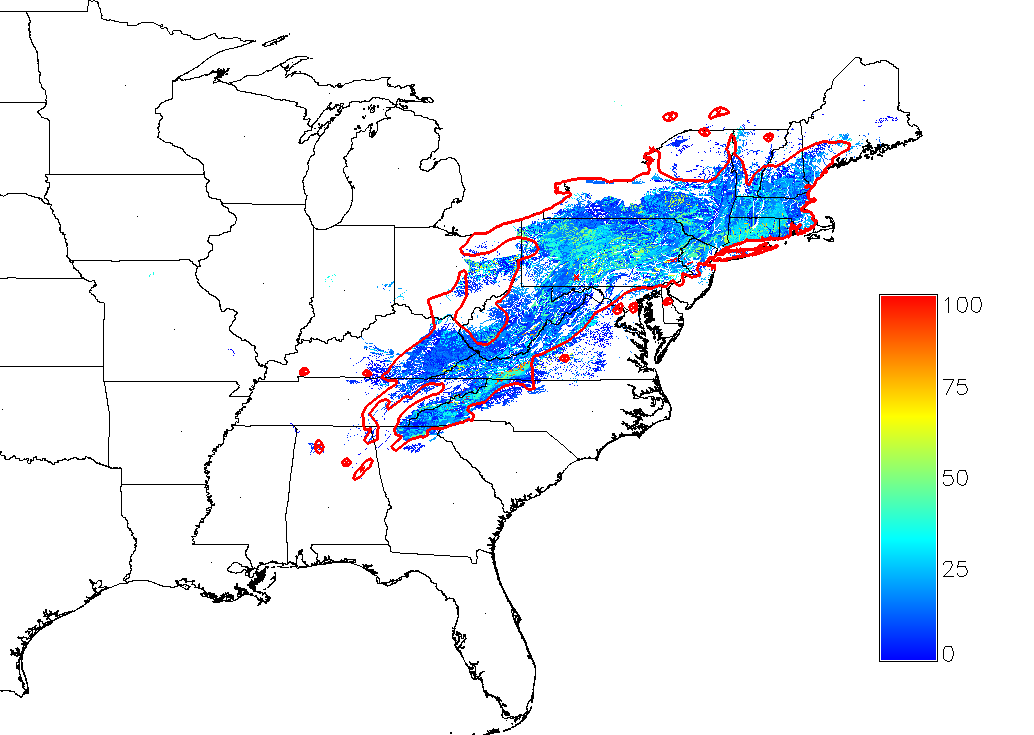
\includegraphics[width=0.47\textwidth]{tree_ranges_figures/Betula_lenta_interpolatedIV_0_cropped.png} &
  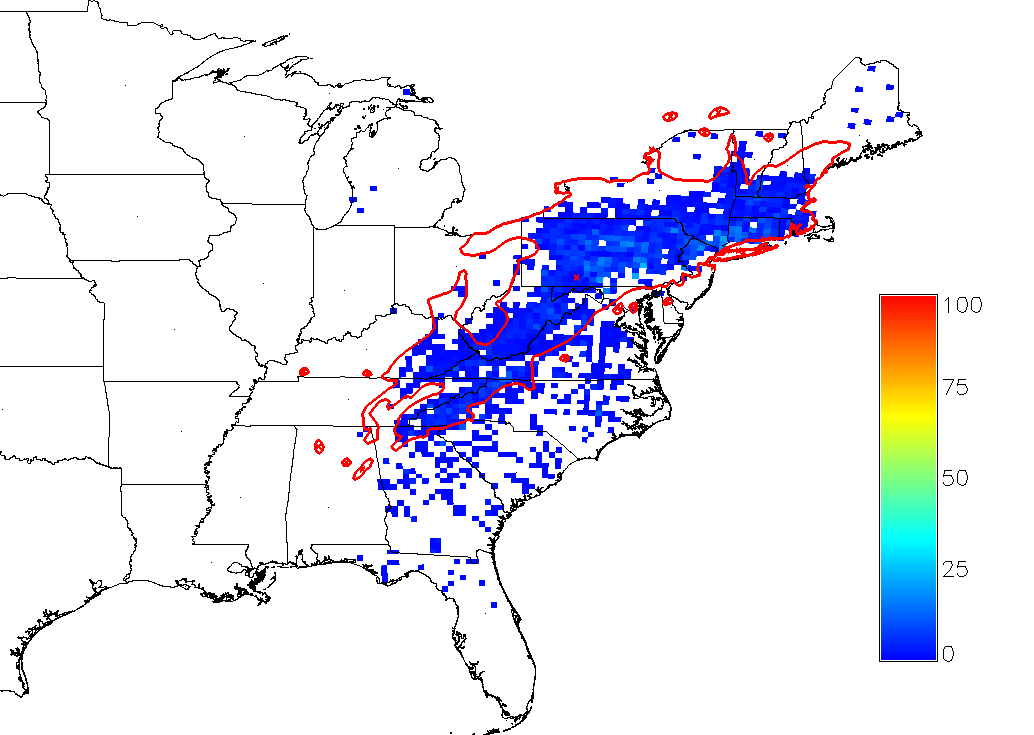
\includegraphics[width=0.47\textwidth]{tree_ranges_figures/Betula_lenta_interpolatedIV_1_cropped.png} \\
   & & Clustering (Kumar et al., in prep.) & \citet{Prasad_Ecosystems_20060301} \& \citet{Iverson_ForestEcolManag_20080210} \\
  \begin{sideways} Flowering Dogwood \end{sideways} &
  \begin{sideways} (\textit{Cornus florida}) \end{sideways} &
  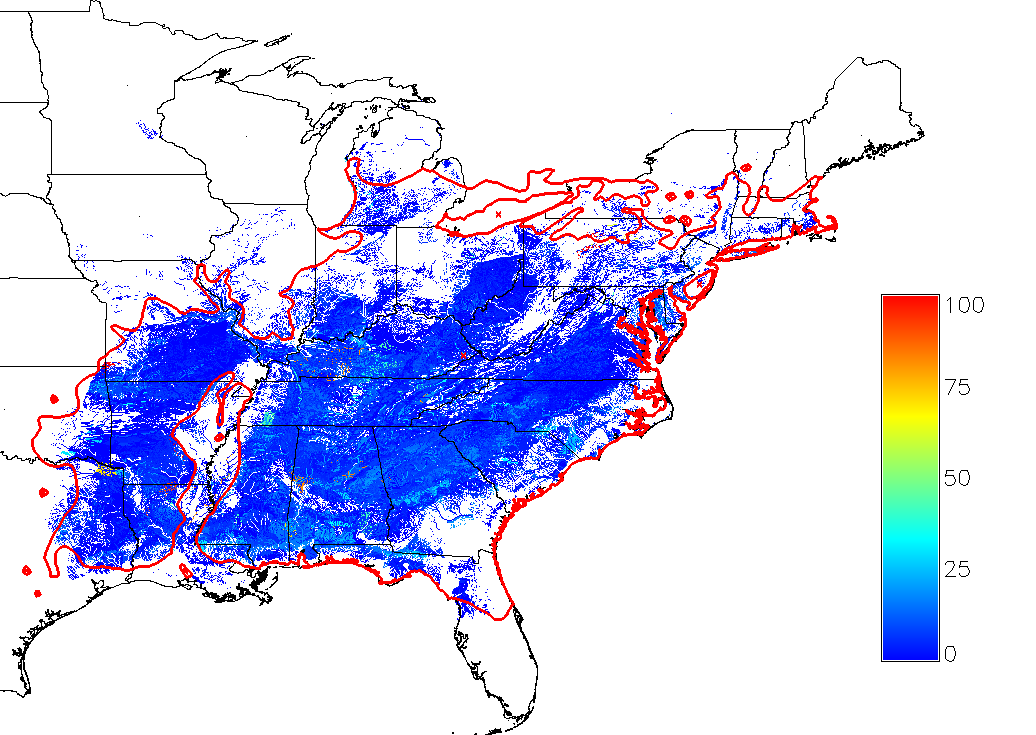
\includegraphics[width=0.47\textwidth]{tree_ranges_figures/Cornus_florida_interpolatedIV_0_cropped.png} &
  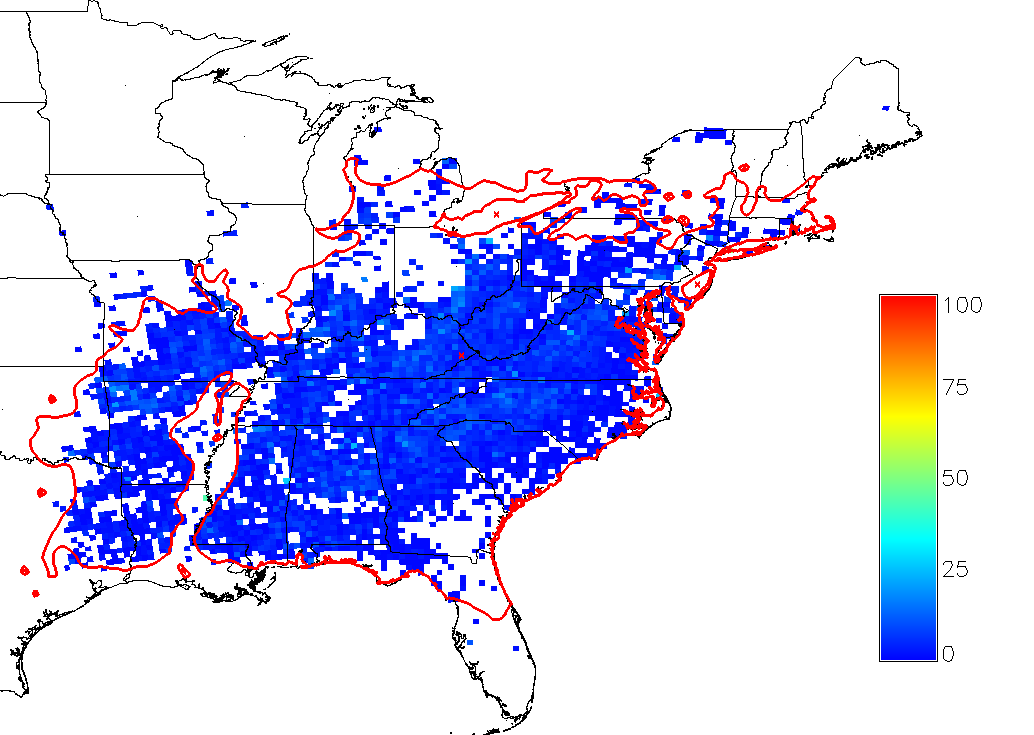
\includegraphics[width=0.47\textwidth]{tree_ranges_figures/Cornus_florida_interpolatedIV_1_cropped.png} \\
   & & Clustering (Kumar et al., in prep.) & \citet{Prasad_Ecosystems_20060301} \& \citet{Iverson_ForestEcolManag_20080210} \\
 \end{tabular}
\end{frame}
%%%%%%%%%%%%%%%%%%%%%%%%%%%%%%%%%%%%%%%%%%%%%%%%%%%%%%%%%%%%%%%%%%%%%%%%%%%%%%%
